\section{Problem-Analyse}

In diesem Abschnitt werden die Probleme beschrieben, die bei der Erstellung von Informations- und Kommunikationsmedien in Zusammenhang mit den dargestellten Texten auftreten. Nach der Definition der im Rahmen dieser Bachelor-Thesis verwendeten Begriffe wird die Besonderheit von Text erläutert,  typische Probleme aufgezeigt und mit Beispielen aus der Praxis belegt.

\subsection{Definition}
\label{l:def}

In dieser Bachelor-Thesis werden bestimmte allgemeine Begriffe und deren Synonyme verwendet, deren konkrete Bedeutung im Kontext dieser Arbeit wie folgt definiert ist:

\paragraph{Workflow (Ablauf)} Die Automatisierung eines Business-Prozesses, als Ganzes oder in Teilen, in welchem Dokumente, Informationen oder Aufgaben entsprechend einer Menge von prozeduralen Regeln von einem zum anderen Teilnehmer zur Bearbeitung weitergegeben werden \cite[S.8]{wmc}. Allgemein lässt sich sagen, dass ein Workflow aus den zum Erreichen eines Zieles nötigen Arbeitsschritten besteht.

\paragraph{Medium (Medien-Produkt, Produkt)} Medien sind physische oder elektronische Informationsträger. Diese Bachelor-Thesis beschäftigt sich vor allem mit Informations- und Kommunikationsmedien und hierbei vor allem mit Massenkommunikationsmitteln, sowohl physischer als auch technischer Natur (vgl. \cite[S.199–201]{schanze2002metzler}). Dies können z.B. Marketingmedien wie Broschüren oder Fernsehwerbespots sein aber auch softwarebasierte Produkte wie eine Smartphone-Anwendungen oder eine Internetseiten. 

\paragraph{Text (Textbaustein)} Damit sind die kleinsten sinnvoll identifizierbaren Bestandteile gemeint, aus denen sich der Text eines Produktes zusammensetzt. Dies sind in der Regel einzelne Sätze bei Druckmedien, können aber auch einzelne Worte sein, wie z.B. die Beschriftung einer Schaltfläche in einer Anwendung.

\paragraph{Agentur} Ein Unternehmen das Medien erstellt. In der Regel sind dies Werbeagenturen, Medien-Produktionsfirmen oder Software-Systemhäuser. 

\paragraph{Projekt} Die Erstellung von Medien erfolgt in Agenturen in Projektarbeit. Projekte sind zeitlich begrenzt und vereinen zielgerichtet die zur Erstellung des Produktes beteiligten Mitarbeiter und Ressourcen. 

\paragraph{Kunde} Ein Unternehmen das Agenturen mit der Erstellung von Medien beauftragt.

\paragraph{Werkzeug (Anwendung)} Eine Software, die eine spezielle Funktion erfüllt. Adobe Photoshop ist ein Werkzeug zur Bearbeitung von Bildern.

\subsection{Die besondere Rolle von Text in Informations- und Kommunikationsmedien}

Es existieren nahezu keine Medien, die ohne Texte auskommen, denn Text ist im Gegensatz zu Grafiken, Fotos oder Animationen ein eindeutiger Informationsträger und unterliegt viel weniger stark einer Interpretation durch den Rezipienten eines Mediums als die symbolisierte oder stilisierte Darstellung von Informationen in audiovisuellen Medien. Text wird in der Marketing-Kommunikation als Unterstützung der zu übermittelnden Information verwendet. Hat man die Aufmerksamkeit des Betrachter eines Produkts erlangt, liefert Text weitere Informationen zum Produkt, er dient dazu, die emotionale Botschaft zu erläutern und zu präzisieren. Auch aus rechtlichen Aspekten ist Text aus den genannten Gründen der einzige verbindliche Informationsträger – bestes Beispiel hierfür ist das sogenannte \typoquotes{Kleingedruckte}, dass sich gerade bei inhaltlich sehr stark komprimierten Werbeformen, wie z.B. Plakat- oder Fernsehwerbung, findet. Ist die Textmenge, die in der Marketing-Kommunikation zum Einsatz kommt, noch überschaubar, gibt es doch Medien die hauptsächlich aus Text bestehen. Hierunter fallen klassische Druckerzeugnisse wie Broschüren und Kataloge oder Produkte der Unternehmenskommunikation wie Jahresberichte und Pressemeldungen. Besonders digitale Medien werden oft mit großen Textmengen versehen – von der einfachen Produkt-Microsite, über Werbemittel wie Newsletter bis zur Unternehmenswebsite – die Möglichkeit Inhalte hierarchisch zu strukturieren und sogar über eine Suche zugänglich zu machen hebt eine Limitierung des Umfanges, wie bei Druckprodukten, praktisch auf.

\begin{figure}[htb]
\begin{center}
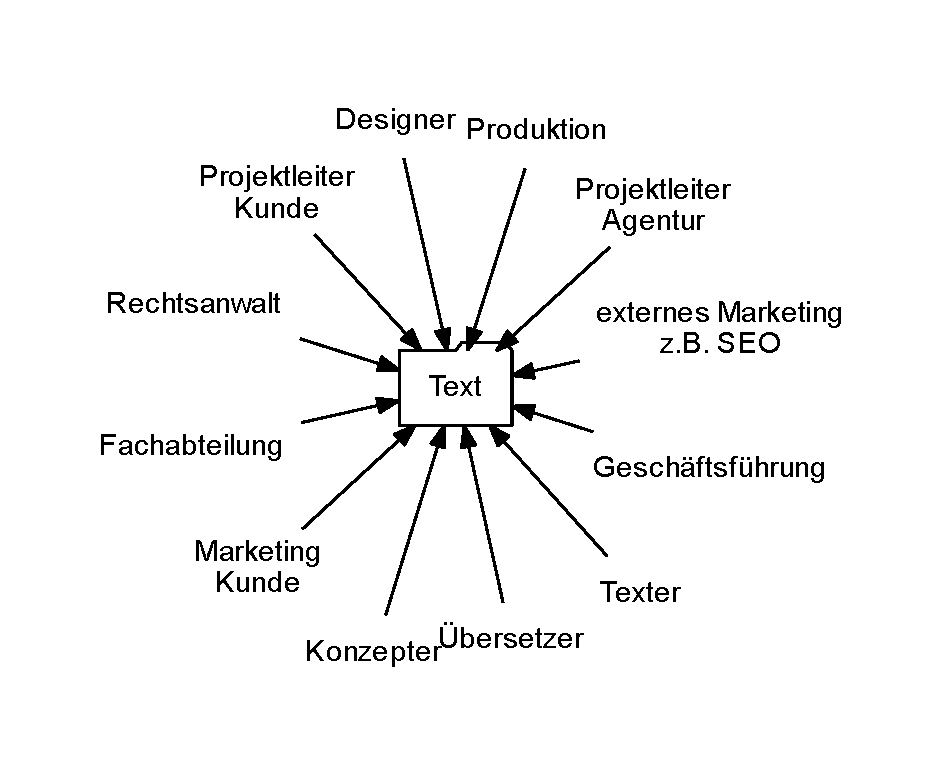
\includegraphics[width=\textwidth]{media/chart-2.pdf}
\end{center}
\caption{Bei der Erstellung von Texten beteiligte Personen}
\label{chart:2}
\end{figure}

Betrachtet man die Abläufe von Projekten, in deren Verlauf Medien erstellt werden, lassen sich bezüglich der Textbestandteile dieser Produkte immer wieder sehr ähnliche Vorgehensweisen und Besonderheiten beobachten. Aufgrund der verbindlichen Natur von Text sind an der Erstellung der Texte für das Medium mehr Personen beteiligt, als es z.B. für die Gestaltung, der Auswahl von Bildmaterial oder für die Programmierung der Fall ist,  da er sehr viele verschieden Kriterien erfüllen muss. Tabelle~\ref{table:textkriterien} auf Seite~\pageref{table:textkriterien} listet exemplarisch eine typische Gruppe von Personen auf, die im Verlauf eines Projektes Einfluss auf den Text eines Produktes haben. Dieser Einfluss wird dabei in der Regel nicht in einer sinnvollen Reihenfolge und im Sinne des geplanten Projektverlaufes ausgeübt. Gerade auf die Mitarbeiter auf Kundenseite haben Agenturen keinen Einfluss; in Projektplänen lassen sich zwar verbindliche Termine für die Lieferung von Texten des Kunden festlegen, dies verhindert aber keinesfalls, dass zu einem späteren Zeitpunkt Änderungen notwendig werden – Hinweise von Anwälten sollten im besten Fall \emph{vor} einer Übersetzung vorliegen, richtet sich aber nach ihren eigenen Terminplänen. Auch die Kriterien wie Text beeinflusst wird, sind sehr vielfältig: Im Entwurf und in der Umsetzung der Produkte legen Designer, Architekten und Produzenten die Struktur von Text wie Art der Ansprache, maximale Wortlänge, Anzahl der Wörter einer Überschrift fest oder diese werden durch das verwendete Medium vorgegeben, Texter legen die Inhalte fest, die wiederum durch Wünsche des Kunden beeinflusst werden; das Lektorat, Fachabteilungen und Anwälte begutachten die Texte dann bezüglich der jeweils erforderlichen Korrektheit.

\begin{table}
\begin{center}
\begin{tabular}{@{}l l l l}
\textbf{Kriterium} & \textbf{Art} & \textbf{Verantwortlich} & \textbf{Organisation}\\
\hline
Aufgabenverteilung & Mitarbeiter & Projektleiter & Agentur\\
\hline
Zielgruppe & Struktur & Informationsarchitektur & Agentur\\
\hline
Umfang, Satzlänge & Struktur & Art-Direktion & Agentur\\
\hline
Länge einzelner Wörter & Struktur & Programmierer & Agentur\\
\hline
Information & Inhalt & Texter & Extern\\
\hline
Orthographie & Korrektheit & Lektorat & Extern\\
\hline
Übersetzung & Sprache & Übersetzungsbüro & Extern\\
\hline
Suchmaschinen-Optimierung & Inhalt & SEO-Experte & Extern\\
\hline
Aufgabenverteilung & Mitarbeiter & Projektleiter & Kunde\\
\hline
Fachliche Aspekte & Korrektheit & Fachabteilung & Kunde\\
\hline
Rechtliche Aspekte & Korrektheit & Rechtsanwalt & Kunde\\
\hline
Werbeaussagen & Inhalt & Marketingabteilung & Kunde\\
\hline
… & … & …
\end{tabular}
\caption{Kriteren von Textbausteinen und verantwortliche Personen}
\label{table:textkriterien}
\end{center}
\end{table}

Wie man Tabelle~\ref{table:textkriterien} entnehmen kann, existieren vielfältige Einflussmöglichkeiten auf die Gestaltung von Texten für Medien die sich auf viele Verantwortliche verteilen. Der Grund dafür ist, dass alle Beteiligten jeweils spezifisches Fachwissen in den Text einfließen lassen, seien es gestalterische Aspekte, die Einfluss auf die Struktur haben, oder das wissen über exakte technische Abläufe, die nur Spezialisten in den Fachabteilungen auf Kundenseite bekannt sind. Dieses Expertenwissen kann nicht für die meist kurze Projektlaufzeit an die umsetzenden Agentur vermittelt werden. Es ist also unvermeidlich, dass Text während des gesamten Projektverlauf geändert werden kann. Neben den Einflüssen durch Experten gibt es auch projektbedingte Einflüsse auf Text in letzter Minute. Sind in Texten Informationen enthalten sind, die einen zeitlichen Aspekt abbilden, ergeben sich durch Verzögerungen im Projekt automatisch Änderungsanforderungen. Ein Beispiel sind Gewinnspiele: Verschiebt sich durch Probleme während dem Projekt der Zeitpunkt, ab dem ein Produkt beim Rezipienten vorliegt, müssen auch eventuell knapp kalkulierte Gewinnspieltermine angepasst werden. Ein weiterer Grund für vielfältige Textänderungen im Verlauf eines Projektes ist die Erwartungshaltung des Kunden – da es Kunden aus ihrem eigenen Arbeitsalltag gewöhnt sind, mit Textverarbeitungsprogramme zu arbeiten, und sie so aus eigener Erfahrung vermeintlich wissen dass Texte schnell geändert sind, erwarten sie auch, dass die Texte im Produkt bis zum Schluss geändert werden können; ihnen ist nicht bewusst, das vom ursprünglichen Text im Quelldokument bis zur Darstellung im fertigen Produkt viele aufwändige Arbeitsschritte nötig sein können.

\bigskip

In diesem Abschnitt wurde gezeigt, das Texte in Medien durch viele Personen und über den gesamten Verlauf eines Projektes geändert werden können. Im nächsten Abschnitt wird erläutert, wie der Austausch über diese Textänderungen erfolgt und welche Probleme dabei entstehen.

\subsection{Das Werkzeug der Wahl zur Verwaltung von Text: \emph{Microsoft Office}}

Zur Abbildung der komplexen Abläufe bei der Erstellung von Informations- und Kommunikationsmedien liefern etablierte Software-Hersteller passende Lösungen. auch speziell für Texte: Mit \emph{InCopy} liefert \emph{Adobe} eine \typoquotes{Lösung für Texterstellung und -bearbeitung, die aufgrund der engen Integration mit Adobe InDesign® CS5.5 effektivere Zusammenarbeit zwischen Redakteuren und Layoutern ermöglicht} \cite{adobeincopy} und  die \emph{Content Station} von \emph{Woodwing} \typoquotes{ist […] eine einzige Oberfläche für alle Schritte des Publishing-Prozesses. […] Unter Nutzung der Desktop- oder der Web-Version können die Team-Mitglieder unabhängig ihres Aufenthaltsorts mitarbeiten} \cite{woodwing} – um nur zwei Beispiele zu nennen. Doch obwohl spezialisierte Werkzeuge existieren finden man diese in Agenturen nur selten – das Werkzeug der Wahl zur Verwaltung der Texte ist in den allermeisten Fällen eine in der Agentur vorhandene Textverarbeitungs- oder Tabellenkalkulationssoftware, in den allermeisten Fällen handelt es sich dabei um den Marktführer in diesem Bereich, \emph{Microsoft} \emph{Word} oder \emph{Excel}. Angesichts des komplizierten Workflows in Projekten und dem Vorhandensein dafür speziell entwickelter Werkzeuge, ist der Einsatz von \emph{Word} oder \emph{Excel} statt dessen fragwürdig und muss genauer betrachtet werden. 

% MARK

Textverarbeitungsprogramme verfügen über viele der für den Text-Workflow benötigten Funktionen:  

\begin{itemize}
\item{Strukturierung von Texten}
\item{Rechtschreibkorrektur für alle gängigen Sprachen}
\item{Kommentarfunktion}
\item{Änderungsfunktionen (Nachverfolgen, wer was geändert hat)}
\item{Möglichkeit zur hierarchischen Strukturierung der Texte in Seiten, Kapitel und Abschnitte}
\item{Möglichkeit zum Anlegen eines Inhaltsverzeichnisses (in Word)
die tabellarische Ansicht in Excel ermöglicht eine übersichtliche Darstellung, meist mit der Originalsprache in der ganz linken Spalte, pro Zeile ein Text, die Übersetzungen dann in den weiteren Spalten}
\item{Export-Funktion nach PDF}
\item{Globales Suchen und Ersetzen}
\item{Formatierungsfunktionen (fett, kursiv, farblich) zum Hervorheben von wichtigen Passagen oder Markieren von Todos, etc.}
\item{Setzen von Hyperlinks (für Web-Projekte)}
\end{itemize}

Auch im Hinblick auf nicht-funktionale Aspekte bieten Textverarbeitungsprogramme einige Vorteile, sind sie doch in den allermeisten Unternehmen der Standard zur Textverarbeitung und sogar plattformunabhängig verfügbar – zumindest existiert die Möglichkeit das Microsoft Office-Dateiformat auf allen Plattformen zu bearbeiten. Da bei allen Projektbeteiligten eine Installation von \emph{Microsoft Office} vorausgesetzt werden kann, werden sie zu \typoquotes{leichtgewichtige} Werkzeugen, die vom Anwender keine zusätzlichen Aufwände z.B. bei der Installation oder Eingewöhnung erfordern. Selbst auf Plattformen, die von \emph{Microsoft Office} nicht offiziell unterstützt werden (z.B. Linux) existieren Programme mit denen das Office-Dokumenten-Format geöffnet und bearbeitet werden kann. Als Standard-Software im Business-Bereich sind alle Beteiligten an diese Software und ihre Funktionen gewöhnt, eine möglicherweise Aufwändige Einweisung in ein weiteres Werkzeug entfällt. Office-Dateien sind einfach auszutauschen – in Unternehmen werden die Dateien in der Regel auf einem Netzwerk-Laufwerk gespeichert. Zum Bearbeiten legt man sich eine lokale Kopie an und arbeitet in dieser Datei. Anschließend kopiert man die neue Version, meist unter Einhaltung eines bestimmten Benamungsschemas, wieder auf dem Netzlaufwerk ab. Hier können Konflikte auftreten (wenn zwei Personen gleichzeitig an der selben Datei arbeiten), diese müssen dann manuell gelöst werden. Wird die Datei direkt vom Netzlaufwerk geöffnet wird diese gesperrt und kann nur von einer Person bearbeitet werden.

Aufgrund der scheinbaren Vorteile der Office-Suite wird diese zu Beginn eines Projektes als geeignet angesehen und als Werkzeug für die Erfassung, Definition und Übersetzung der Texte eines Projektes ausgewählt. Im alltäglichen Gebrauch treten viele Probleme gerade im Bereich des gemeinsamen Bearbeitens, paralleler oder nachträglicher Änderungen und der Übertragung der fertigen Texte in den Produktionsprozess auf. Die im Verlauf des Projekts auftauchenden Probleme werden dann als gegeben akzeptiert, da man \typoquotes{nun} damit zurecht kommen muss, um den Verlauf des Projektes nicht zu verzögern. Bei neuen Projekten wird aber die gleiche Entscheidung wieder getroffen.

% Bis vorige MARK überarbeiten
% MARK

\subsection{Office-Programme sind die falschen Werkzeuge}

% Stimmt so nicht mehr, habe oben gezeigt, DASS es Lösungen gibt.
% Problem ist mangelnde Akzeptanz, bzw. Fehlentscheidung
% Eigentlich muss mich das aber gar nicht so sehr interessieren,
% ich will in dieser Arbeit niemanden überzeugen sondern einfach 
% eine Lösung bieten (aber schon darauf eingehen)

Der Grund, warum Office-Programme wie \emph{Word} und \emph{Excel} verwendet werden ist der, dass keine keine dedizierten Lösungen existieren, die explizit die genannten Abläufe in der Textverarbeitung abbildet. Es existieren vielen Produkte aus dem Bereich der Projektverwaltungswerkzeuge, Mediendatenbanken oder Content-Management-Systemen die die Prozesse rund um die Erstellung von Informations- und Kommunikationsmedien vereinfachen, aber keine kann die genannten Probleme und Abläufe zufriedenstellend abbilden.

\subsection{Beispiele aus der Praxis}

Die Analyse des Problems basiert auf Interviews mit Menschen, die in ihrem Arbeitsalltag regelmäßig mit Texten zu tun haben. In diesen Interviews wurden die Personen nach ihren Erfahrungen in der Projektarbeit bezüglich Texten befragt und gebeten die aus ihrer Sicht am häufigsten auftretenden Probleme zu nennen.

\subsubsection{MAN Truck \& Bus AG: Texte für mobile Vertriebssoftware}

Markus Rüb ist als Projektleiter bei der MAN Truck \& Bus AG mit der Einführung von Tablet-PCs als Vertriebshilfsmittel betraut.

\subsection{Schlussfolgerung}

